\chapter{Performance Evaluation}
\label{chap:performance-evaluation}
\centerline{\rule{149mm}{.02in}}
\vspace{2cm}

TODO

\section{Performance Timings}

TODO

\section{Memory Overhead}

TODO

\section{Impact of Bucket Size}

TODO

\section{Impact of Tree Balance}

TODO

\section{Summary}

TODO




\subsection{Real Datasets and Impact of Bucket Size}

\begin{table}
	\centering
	\makebox[\textwidth][c]{%
		\begin{tabular}{|r|r|l|l|l|}
			\hline
			\multicolumn{2}{|c}{} & \multicolumn{3}{|c|}{\textbf{Dataset}} \\
			\hline
			\textbf{Structure} & \textbf{Operation} & \textbf{Astrophysics} & \textbf{Hurricane Isabel} & \textbf{Armadillo Mesh} \\
			\hline
			\multirow{4}{*}{Sequential Scan} & Delete & 1315.81 & 1920.73 & 1336.2 \\
				& Insert & 436.385 & 691.833 & 215.865 \\
				& Point Query & 435.88 & 651.428 & 212.585 \\
			\hline
			\multirow{4}{*}{Rebuild Index PPT} & Delete & 1856.11 & 2121.9 & 36.0037 \\
				& Insert & 139.346 & 117.441 & 0.112088 \\
				& Point Query & 139.048 & 117.292 & 0.0492687 \\
			\hline
			\multirow{4}{*}{Bucket PPT} & Delete & 82.908 & 14.9052 & 0.160532 \\
				& Insert & 81.231 & 14.4715 & 0.126938 \\
				& Point Query & 70.4391 & 14.3358 & 0.0956872 \\
			\hline
			\multirow{4}{*}{Splay PPT} & Delete & 88.4574 & 15.3893 & 0.203571 \\
				& Insert & 84.0908 & 14.7177 & 0.192196 \\
				& Point Query & 70.3729 & 14.6499 & 0.141219 \\
			\hline
		\end{tabular}
	}%

	\caption{Total Execution Time (in seconds) of Each Operation on Real Datasets}
	\label{tab:perf1-real}
\end{table}

Table \ref{tab:perf1-real} shows the runtime of each operation on sampled real datasets. Work gone into increasing the speed of the Pseudo-Pyramid Tree by exploring different implementations, which has worked to greatly accelerate the structure for most of the evaluation datasets. However, Table \ref{tab:perf1-real} shows that on the two scientific datasets, the relative speedup from Sequential Scan achieved by the Bucket Pseudo-Pyramid Tree appears low.

For example, $500,000$ point queries with the astrophysics dataset takes 435.88 seconds with Sequential Scan and 70.4391 seconds with the Bucket Pseudo-Pyramid Tree, meaning a speedup of $\frac{435.88}{70.4391} \approx 6.18$ has been achieved. Speedup for the hurricane Isabel dataset is slightly higher, being approximately 45.44. Compare these figures to the speedup gained with the armadillo mesh, which is 2221. With such a high speedup on some datasets, and the fact there exist algorithms which can perform search in $O(log_2 n)$ time, this raised an important question: why the speedup is so low?

Despite hashing a point taking $O(d)$ time, point queries will take much longer if there are large numbers of points in buckets. If each bucket contains exactly one point, then the complexity approaches $O(d)$. On the other extreme, where a single bucket contains all points, the complexity becomes $O(n)$. The number of points in a bucket, or \textit{bucket size}, is one of the most important factors to consider when analysing the performance of hash-based index structures. A ``good" hashing function tries to achieve an amortised running time of $O(1)$ by ensuring only one or two points are mapped to the same hash value.

\begin{table}
	\centering
	\begin{tabular}{|l|l|l|l|l|}
		\hline
		& & \multicolumn{3}{c|}{\textbf{Bucket Size Statistics}} \\
		\hline
		\textbf{Dataset} & \textbf{Time to Query (sec)} & \textbf{Average} & \textbf{Max} & \textbf{\#Buckets} \\
		\hline
		500,000 16D Random Points & 0.105091 & 1.0312 & 4 & 493488 \\
		500,000 Astrophysics Points & 70.4391 & 47820.89 & 153471 & 8  \\
		500,000 Hurricane Isabel Points & 14.3358 & 1257.46 & 154979 & 396 \\
		435,544 3D Armadillo Mesh Points & 0.141219 & 19.1465 & 187 & 22748 \\
		\hline
	\end{tabular}
	\caption{Statistics on Bucket Size with Pseudo-Pyramid Tree Based on Dataset}
	\label{tab:perf1-bucket-stats}
\end{table}

The mean, standard deviation, minimum and maximum bucket size has been used to determine if bucket size is the reason the Pseudo-Pyramid Tree is so slow for the astrophysics dataset. Table \ref{tab:perf1-bucket-stats} shows these statistics when the Pseudo-Pyramid Tree is storing points from one synthetic dataset and all the real datasets. There appears to be a relationship between average bucket size and the speed of the Pseudo-Pyramid Tree. The average bucket size for the scientific datasets go into the thousands for the scientific datasets, with the largest bucket containing 153471 and 497953 points using the astrophysics and hurricane datasets respectively. Notice how the time to query all points in the 16D random dataset takes the shorter time, due to the average bucket size being as small as 1.0312. These results match the observation that larger average bucket size means more computation must be performed per operation on average.










\subsection{Bucket Statistics}
\label{sec:bucket-stats}

The same underlying implementation is used for the Pseudo-Pyramid Tree, Pyramid Tree and Bucket Hash Table. Only how the hashing function allocates points to buckets varies. Pyramid Tree's and Bucket Hash Table's hash functions have also been parallelised using SSE, which has made the difference between execution times of the individual hash functions of the three structures very small, allowing for a fair comparison of execution time.

\begin{table}
	\centering
	\makebox[\textwidth][c]{%
		\begin{tabular}{|l|l|l|l|l|}
			\hline
			& & \multicolumn{3}{c|}{\textbf{Bucket Size Statistics}} \\
			\hline
			\textbf{Dataset} & \textbf{Time to Query (sec)} & \textbf{Average} & \textbf{Max} & \textbf{\#Buckets} \\
			\hline
			\textbf{Pseudo-Pyramid Tree} & & & & \\
			500,000 16D Random Points & 0.105091 & 1.0312 & 4 & 493488 \\
			500,000 Astrophysics Points & 70.4391 & 47820.89 & 153471 & 8  \\
			500,000 Hurricane Isabel Points & 14.3358 & 1257.46 & 154979 & 396 \\
			435,544 3D Armadillo Mesh Points & 0.141219 & 19.1465 & 187 & 22748 \\
			\hline
			\textbf{Pyramid Tree} & & & & \\
			500,000 16D Random Points & 0.177153 & 1.16285 & 7 & 429974 \\
			500,000 Astrophysics Points & 60.0216 & 3586.57 & 235260 & 120 \\
			500,000 Hurricane Isabel Points & 44.1224 & 4048.4 & 354965 & 123 \\
			435,544 3D Armadillo Mesh Points & 0.13448 & 2.45933 & 1173 & 177095 \\
			\hline
			\textbf{Bucket Hash Table} & & & & \\
			500,000 16D Random Points & 0.249102 & 1.01004 & 3 & 495172 \\
			500,000 Astrophysics Points & 0.172516 & 1.01057 & 5 & 425002 \\
			500,000 Hurricane Isabel Points & 0.222288 & 1.00987 & 3 & 493081 \\
			435,544 3D Armadillo Mesh Points & 0.0811833 & 1.00857 & 3 & 431696 \\
			\hline
		\end{tabular}
	}%
	\caption{Statistics on Bucket Size, Based on Dataset, of All Hash-Based Structures}
	\label{tab:perf2-bucket-stats}
\end{table}

Since the implementation details of the three structures are similar, the bucket size will be used to compare the structures. Table \ref{tab:perf2-bucket-stats} contains statistics on bucket size of all three hashing functions, using all real datasets and the 16D synthetic dataset.

From these results it is clear that the core factor which determines the performance of each structure is bucket size. The Pseudo-Pyramid Tree and Pyramid Tree have much larger buckets when storing the scientific datasets compared to when they store the synthetic dataset or armadillo mesh. With hurricane Isabel, one bucket in the Pyramid Tree is as large as 497,953, causing it degenerate to semi-sequential scan. When the average bucket size tends to one, all the structures can query all the points in the dataset in less than a half a second.






\subsection{Performance Timings}

\begin{figure}
	\makebox[\textwidth][c]{%
		\begin{subfloat}[\texttt{insert}\label{fig:perf3-dimensionality-insert}]{%
			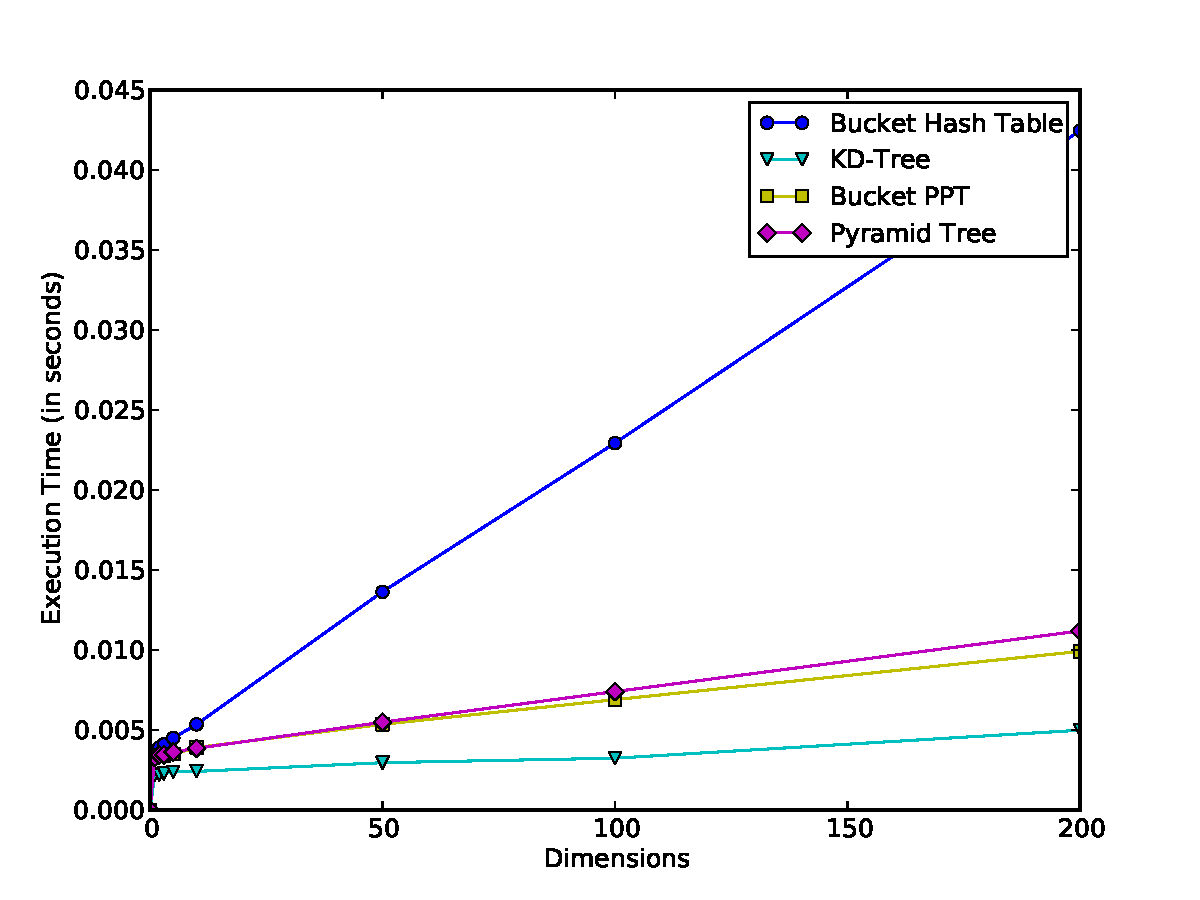
\includegraphics[scale=0.5]{figures/performance_analysis/iteration_3/randuniform_insert.pdf}
		}
		\end{subfloat}
		\begin{subfloat}[\texttt{delete}\label{fig:perf3-dimensionality-remove}]{%
			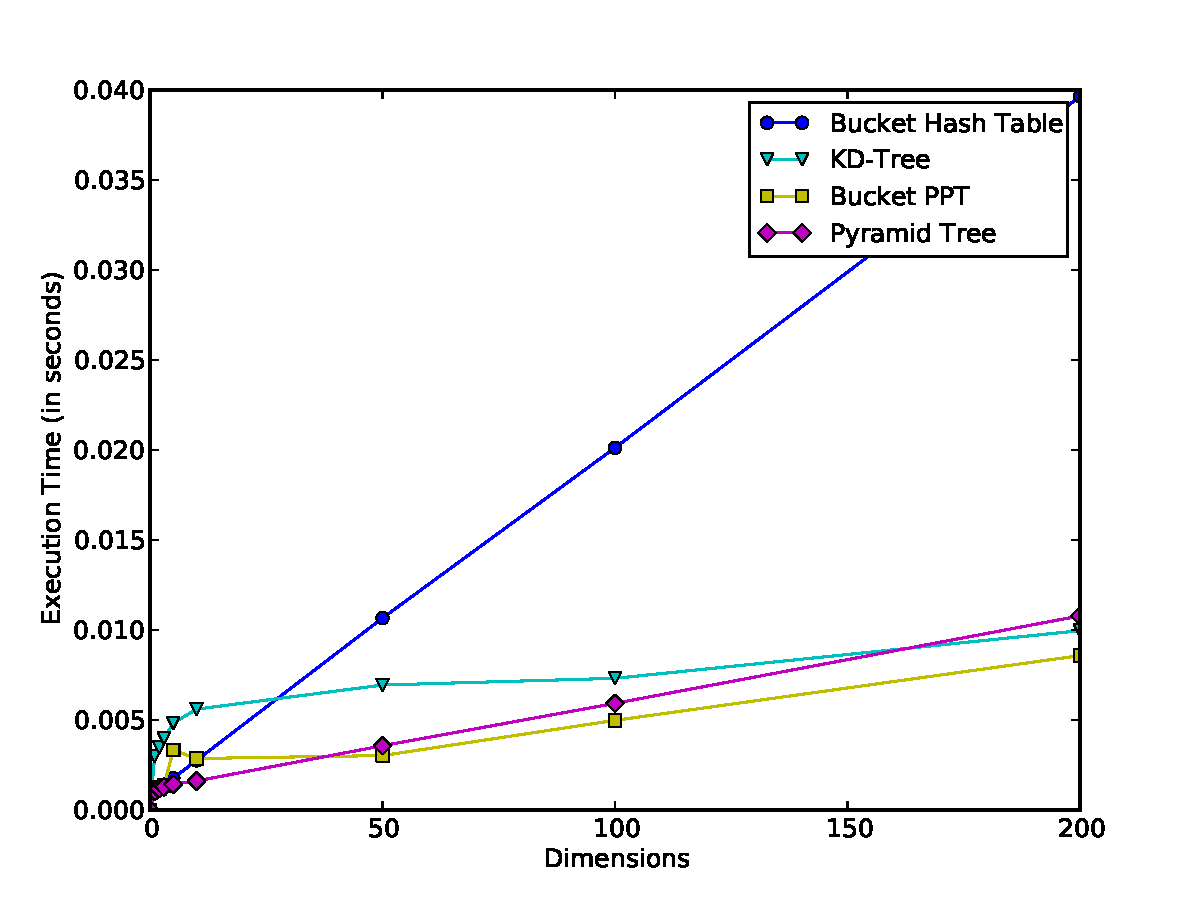
\includegraphics[scale=0.5]{figures/performance_analysis/iteration_3/randuniform_delete.pdf}
		}
		\end{subfloat}
	}%

	\caption{Index Structure Performance With Respect To Dimensionality (10,000 Points from Uniform Distribution Synthetic Dataset)}
	\label{fig:perf3-dimensionality}
\end{figure}

\begin{figure}
	\makebox[\textwidth][c]{%
		\begin{subfloat}[\texttt{insert}\label{fig:perf3-size-insert}]{%
			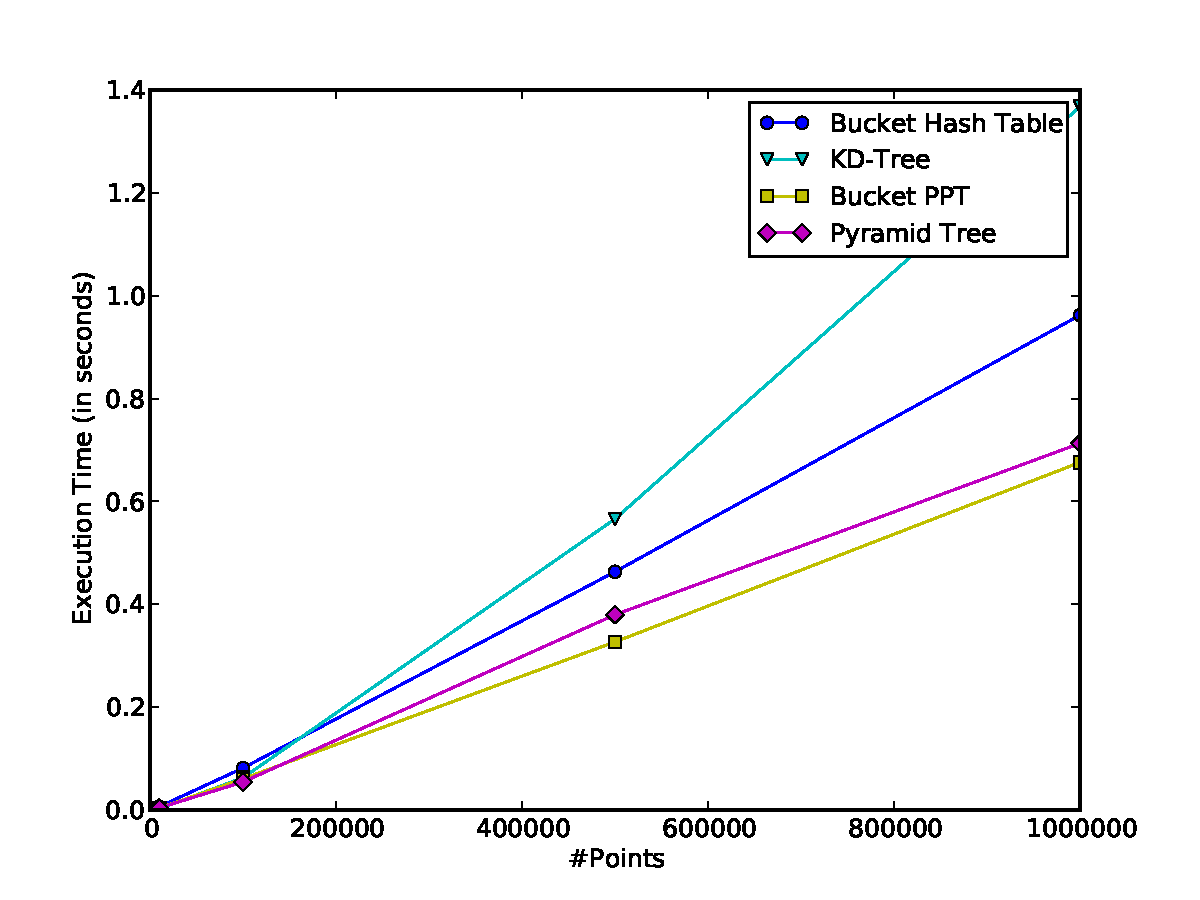
\includegraphics[scale=0.5]{figures/performance_analysis/iteration_3/sizevary_insert.pdf}
		}
		\end{subfloat}
		\begin{subfloat}[\texttt{delete}\label{fig:perf3-size-remove}]{%
			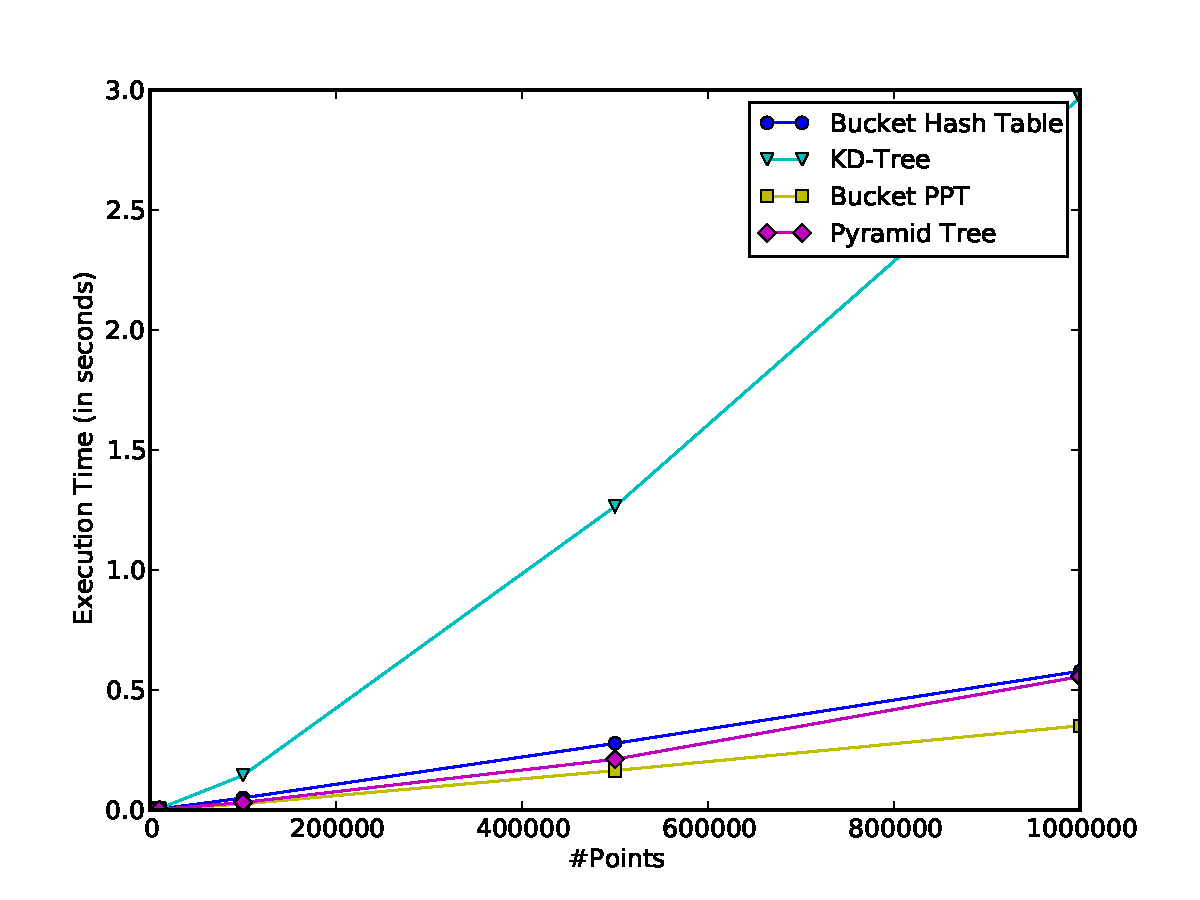
\includegraphics[scale=0.5]{figures/performance_analysis/iteration_3/sizevary_delete.pdf}
		}
		\end{subfloat}
	}%

	\caption{Index Structure Performance With Respect To Dataset Size (10,000 Points from Uniform Distribution Synthetic Dataset)}
	\label{fig:perf3-size}
\end{figure}

Tables containing the total execution times of all three operations of each structure for all synthetic datasets is available in Appendix \ref{sec:appendix-perf3}. Plots with dimension against execution time are shown for \texttt{insert} and \texttt{delete} in Figure \ref{fig:perf3-dimensionality} when processing random points from a uniform distribution.

In general, as $d$ increases the speed of the hash-based structures decreases faster than the $kd$-tree. For insertion, the $kd$-tree consistently outperforms the hash-based structures. For deletion, the $kd$-tree is initially slower but as $d$ increases it starts to beat the hash-based structures. This is most likely because each hashing function takes $O(d)$ time. The $kd$-tree does not require such a function to begin the search and as such, is more resilient to higher-dimensional search for point queries.

The Bucket Hash Table results in lower bucket size at the cost of a more expensive hashing function. Despite having the same complexity, the Pseudo-Pyramid Tree and Pyramid Tree hash functions require less computation (i.e. the constant factor is lower). Since these two structures also result in low average bucket size for synthetic data, they are faster than the Bucket Hash Table for synthetic data. Figure \ref{fig:perf3-dimensionality} illustrates this by showing that the growth in execution time of Bucket Hash Table is the fastest. 

The execution times between the Pyramid Tree and the Pseudo-Pyramid Tree is very small, but the latter structure is consistently faster. Table \ref{tab:perf2-bucket-stats} in Section \ref{sec:bucket-stats} shows that the Pseudo-Pyramid Tree results in lower bucket size for random points generated from a uniform distribution. This combined with the fact the Pseudo-Pyramid Tree function requires slightly less computation makes it faster than the Pyramid Tree.

Execution times for the 16 dimension dataset of varying size is shown in Figure \ref{fig:perf1-size}. While the $kd$-tree performs faster when $d$ is increased, the increase in speed becomes negligible as more points are inserted into the structures. This is especially the case with \texttt{delete}, where execution time grows much faster.

As long as the average bucket size tends to one, the speed of the hash-based structures is higher than the $kd$-tree. Since all three hash-based structures have low average bucket size for the synthetic data, the relative performance of the structures depends on the hashing function itself. Since the Pseudo-Pyramid Tree has the cheapest hashing function, it is the fastest structure for the synthetic datasets.

\subsection{Real Datasets}

\begin{table}
	\centering
	\makebox[\textwidth][c]{%
		\begin{tabular}{|r|r|l|l|l|}
			\hline
			\multicolumn{2}{|c}{} & \multicolumn{3}{|c|}{\textbf{Dataset}} \\
			\hline
			\textbf{Structure} & \textbf{Operation} & \textbf{Astrophysics} & \textbf{Hurricane Isabel} & \textbf{Armadillo Mesh} \\
			\hline
			\multirow{4}{*}{Bucket Hash Table} & Delete & 0.191339 & 0.248544 & 0.102674 \\
				& Insert & 0.360452 & 0.419106 & 0.11828 \\
				& Point Query & 0.172516 & 0.222288 & 0.0811833 \\
			\hline
			\multirow{4}{*}{$kd$-tree} & Delete & 68.9612 & 578.798 & 0.91045 \\
				& Insert & 0.663231 & 0.434781 & 0.384241 \\
				& Point Query & 0.639265 & 0.408527 &  0.374425 \\
			\hline
			\multirow{4}{*}{Bucket PPT} & Delete & 82.908 & 14.9052 & 0.160532 \\
				& Insert & 81.231 & 14.4715 & 0.126938 \\
				& Point Query & 70.4391 & 14.3358 & 0.0956872 \\
			\hline
			\multirow{4}{*}{Pyramid Tree} & Delete & 60.8105 & 41.5488 & 0.164531 \\
				& Insert & 65.0126 & 44.2493 & 0.192165 \\
				& Point Query & 60.0216 & 44.1224 & 0.134481 \\
			\hline
		\end{tabular}
	}%
	\caption{Total Execution Time (in seconds) of Each Operation on Sampled Real Datasets}
	\label{tab:perf3-real}
\end{table}

Table \ref{tab:perf3-real} shows the runtime of each operation on sampled real datasets. Bucket Hash Table is consistently the fastest structure for all operations and data because its average bucket size is always close to one. Again, the Pseudo-Pyramid Tree and Pyramid Tree degenerate to semi-sequential on the two scientific datasets, with the Pyramid Tree performing slightly better than the Pseudo-Pyramid Tree on the astrophysics dataset.

The $kd$-tree is over one hundred times faster than the Pseudo-Pyramid and Pyramid Trees for the scientific datasets for \texttt{insert} and point queries. However, the structure processes these datasets slower than the synthetic data or armadillo mesh. $kd$-tree's \texttt{delete} operation is also the slowest of all the structures, taking over 500 seconds to individually delete all the points from the hurricane dataset.

\subsection{Impact of $kd$-tree Balance}

The performance timings in the previous section show that the $kd$-tree becomes slower with particular datasets. Despite the $kd$-tree storing the same number of points in each of the real datasets, the performance is different. The speed of processing 500,000 points from the astrophysics or hurricane Isabel datasets is much slower than the armadillo mesh or the synthetic datasets. 

The cause of this is most likely the \textit{balance} of the tree. Skewed datasets are known to affect the balance of spatial decomposition trees, resulting in longer paths from the root node to the leaves. To investigate this further, the \textit{balance factor} of the point $kd$-tree, when storing 500,000 points from three synthetic and three real datasets has been measured. The balance factor is defined as the \textit{average} length of a path from the root to a leaf \cite{kdtree-v-bdtree}. A lower balance factor means the $kd$-tree has to visit less nodes on average when performing a point query, so queries will generally be faster. A $kd$-tree is balanced when its balance factor is $\log_2 n$. When $n = 500,000$, the best possible balance factor is $\log_2 (500,000) \approx 19$.

The \textit{exact match query cost}, used to evaluate $kd$-tree variations by Dandamudi and Sorenson \cite{kdtree-v-bdtree}, represents the average number of points visited in the tree for a point query. Higher exact match query cost means the tree has to do more work on average to find a point, making the structure slower.

\begin{table}
	\centering
	\makebox[\textwidth][c]{%
		\begin{tabular}{|l|l|l|l|}
			\hline
			\multicolumn{1}{|c|}{\textbf{Dataset}} & \centrespecialcell{\textbf{Balance} \\ \textbf{Factor}} & \centrespecialcell{\textbf{Max Path} \\ \textbf{Length}} & \centrespecialcell{\textbf{Exact Match} \\ \textbf{Query Cost}} \\
			\hline
			\leftspecialcell{Random 10D Points \\ (Uniform Distribution)} & 24.8285 & 47 & 24.4968 \\
			\leftspecialcell{Random 10D Points \\ (Skewed Distribution)} & 24.9092 & 44 & 24.5714 \\
			\leftspecialcell{Random 10D Points \\ (Clustered Distribution)} & 30.3362 & 57 & 29.9911 \\
			Astrophysics & 32.405 & 120 & 29.7373 \\
			Hurricane Isabel & 47.7236 & 123 & 40.5602 \\
			\hline
		\end{tabular}
	}%
	\caption{Point $kd$-tree Balance Factor and Exact Match Query Cost with 500,000 Points from Various Datasets}
	\label{tab:kdtree-balance-factor}
\end{table}

The balance factor clearly increases as $n$ is increased, so the concern here is how its affected by data distribution. Table \ref{tab:kdtree-balance-factor} contains the balance factor and maximum path length from the root to a leaf when the point $kd$-tree is storing points from datasets with different distributions. It also contains the exact match query cost of querying all the points stored in the $kd$-tree. 

The table shows that the exact match query cost increases as the balance factor does and thus, the average amount of work required to perform a point query. While the $kd$-tree does not degenerate when processing datasets with skew, these results show that these datasets do affect the structure's overall performance. For this reason, many variants of the $kd$-tree have been developed with the goal of reducing the balance factor, such as the BD-Tree \cite{kdtree-v-bdtree} and fair split tree\cite{fair-split-tree}. However, it is beyond the scope of this document to explore these variants here.

\subsection{Summary}

This iteration showed that the point $kd$-tree, even with no attempts to further optimise the structure, significantly outperformed the Pseudo-Pyramid Tree and Pyramid Tree. The point $kd$-tree is slower than the Bucket Hash Table, especially with individual point deletion, but it is more resilient to floating point inaccuracy as it does not rely on a potentially inaccurate hashing function. The timing data from this iteration results in the following observations:
\begin{enumerate}[noitemsep]
	\item if a \textit{reliable} hashing function that produces an average bucket size very close to one can be found, then a structure which is faster than the point $kd$-tree for point queries can be constructed
	\item the point $kd$-tree is affected by point distribution as shown by the increased balance factor and average point query cost when storing the two scientific datasets
	\item individual point deletion from point $kd$-trees is the slower than every hash-based structure implemented
\end{enumerate}

